\chapter{Architettura del Microprocessore 8086}

\section{Introduzione}

Il microprocessore Intel 8086, introdotto nel 1978, rappresenta una pietra miliare nella storia dell'informatica. È il primo processore della famiglia x86, architettura che ancora oggi domina il mercato dei personal computer. Comprendere l'8086 significa gettare le basi per la programmazione a basso livello su processori moderni.

\begin{definizione}
Il \textbf{microprocessore 8086} è una CPU a 16 bit con bus dati a 16 bit e bus indirizzi a 20 bit, capace di indirizzare fino a 1 MB di memoria (2\textsuperscript{20} = 1.048.576 byte).
\end{definizione}

\section{Caratteristiche principali}

\subsection{Specifiche tecniche}

\begin{table}[h]
\centering
\begin{tabular}{ll}
\toprule
\textbf{Caratteristica} & \textbf{Valore} \\
\midrule
Architettura & 16 bit \\
Bus dati & 16 bit \\
Bus indirizzi & 20 bit \\
Memoria indirizzabile & 1 MB (1.048.576 byte) \\
Frequenza clock & 5-10 MHz \\
Registri general purpose & 4 × 16 bit \\
Registri segmento & 4 × 16 bit \\
Numero transistor & 29.000 \\
Tecnologia & NMOS 3 µm \\
\bottomrule
\end{tabular}
\caption{Specifiche tecniche Intel 8086}
\end{table}

\subsection{Organizzazione interna}

L'8086 utilizza un'architettura pipeline a due stadi per migliorare le prestazioni. La \textbf{Bus Interface Unit (BIU)} è responsabile del prelievo delle istruzioni dalla memoria e della loro gestione, permettendo il prefetching di più istruzioni. L'\textbf{Execution Unit (EU)} invece esegue le istruzioni decodificate. Questi due componenti funzionano in parallelo: mentre l'EU esegue un'istruzione, la BIU già precarica la prossima, creando un effetto pipeline che migliora significativamente la velocità di esecuzione.

\begin{center}
\begin{tikzpicture}[
    node distance=1.5cm and 2cm,
    box/.style={rectangle, draw, fill=blue!20, text width=3cm, align=center, minimum height=1cm},
    queue/.style={rectangle, draw, fill=green!20, text width=2cm, align=center, minimum height=0.8cm}
]
    % BIU
    \node[box] (biu) {Bus Interface Unit (BIU)};
    \node[queue, below=of biu] (queue) {Coda Istruzioni\\(6 byte)};
    \node[box, below=of queue] (mem) {Bus Memoria\\(20 bit)};

    % EU
    \node[box, right=of biu] (eu) {Execution Unit (EU)};
    \node[box, below=of eu] (alu) {ALU\\16 bit};
    \node[box, right=of eu] (regs) {Registri};

    % Frecce
    \draw[->] (biu) -- (queue);
    \draw[->] (queue) -- (mem);
    \draw[<->] (queue) -- (eu);
    \draw[->] (eu) -- (alu);
    \draw[<->] (eu) -- (regs);
\end{tikzpicture}
\end{center}

\begin{nota}
La \textbf{coda di istruzioni} (instruction queue) permette alla BIU di precaricare fino a 6 byte di istruzioni mentre la EU esegue l'istruzione corrente. Questo meccanismo di \emph{prefetch} migliora le performance.
\end{nota}

\section{Modalità di funzionamento}

L'8086 può operare in due modalità:

\subsection{Modalità minima}

Sistema monoprocessore dove l'8086 genera autonomamente tutti i segnali di controllo.

\subsection{Modalità massima}

Sistema multiprocessore con coprocessore 8087 (FPU) e controller DMA 8237. Richiede circuiti esterni per la generazione dei segnali.

\section{Memoria segmentata}

L'8086 utilizza un modello di memoria \textbf{segmentata} per indirizzare 1 MB con registri a 16 bit.

\begin{definizione}
Un \textbf{segmento} è un blocco di memoria di massimo 64 KB (2\textsuperscript{16} byte). L'indirizzo fisico viene calcolato combinando un registro segmento e un offset.
\end{definizione}

\subsection{Calcolo indirizzo fisico}

L'indirizzo fisico a 20 bit si ottiene con la formula:

\[
\text{Indirizzo Fisico} = (\text{Segmento} \times 16) + \text{Offset}
\]

Equivalentemente:
\[
\text{Indirizzo Fisico} = (\text{Segmento} \ll 4) + \text{Offset}
\]

\begin{esempio}
Calcolare l'indirizzo fisico per \texttt{DS:SI = 1234h:5678h}:

\begin{align*}
\text{Segmento} &= 1234h \\
\text{Offset} &= 5678h \\
\text{Indirizzo Fisico} &= (1234h \times 10h) + 5678h \\
&= 12340h + 5678h \\
&= 179B8h
\end{align*}

In decimale: $179B8h = 96.696$ byte.
\end{esempio}

\subsection{Rappresentazione grafica}

\begin{center}
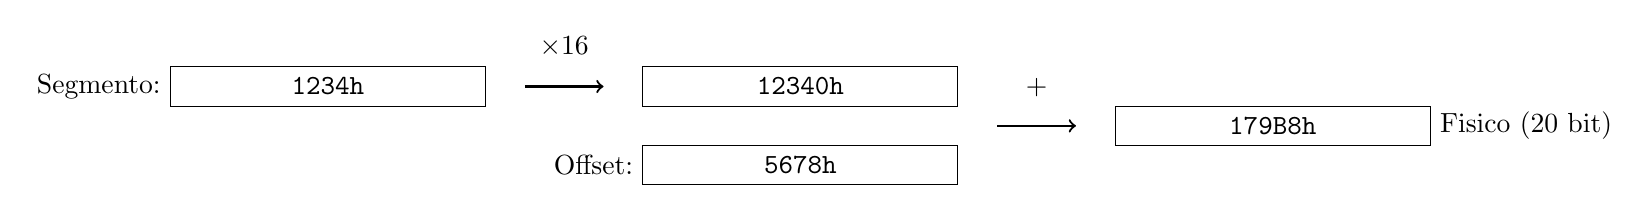
\begin{tikzpicture}
    % Registro segmento
    \draw (0,2) rectangle (4,2.5);
    \node at (2,2.25) {\texttt{1234h}};
    \node[left] at (0,2.25) {Segmento:};

    % Shift left 4 bit
    \draw[->, thick] (4.5,2.25) -- (5.5,2.25);
    \node[above] at (5,2.5) {$\times 16$};

    % Segmento shiftato
    \draw (6,2) rectangle (10,2.5);
    \node at (8,2.25) {\texttt{12340h}};

    % Offset
    \draw (6,1) rectangle (10,1.5);
    \node at (8,1.25) {\texttt{5678h}};
    \node[left] at (6,1.25) {Offset:};

    % Somma
    \draw[->, thick] (10.5,1.75) -- (11.5,1.75);
    \node[above] at (11,2) {$+$};

    % Indirizzo fisico
    \draw (12,1.5) rectangle (16,2);
    \node at (14,1.75) {\texttt{179B8h}};
    \node[right] at (16,1.75) {Fisico (20 bit)};
\end{tikzpicture}
\end{center}

\section{Flag register}

Il registro FLAGS (16 bit) contiene bit di stato e controllo:

\begin{table}[h]
\centering
\small
\begin{tabular}{clp{8cm}}
\toprule
\textbf{Bit} & \textbf{Nome} & \textbf{Descrizione} \\
\midrule
0 & CF & \textbf{Carry Flag}: riporto/prestito in operazioni aritmetiche \\
2 & PF & \textbf{Parity Flag}: parità del byte meno significativo \\
4 & AF & \textbf{Auxiliary Carry}: riporto bit 3 (BCD) \\
6 & ZF & \textbf{Zero Flag}: risultato zero \\
7 & SF & \textbf{Sign Flag}: bit di segno del risultato \\
8 & TF & \textbf{Trap Flag}: modalità debug single-step \\
9 & IF & \textbf{Interrupt Flag}: abilita interrupt mascherabili \\
10 & DF & \textbf{Direction Flag}: direzione operazioni su stringhe \\
11 & OF & \textbf{Overflow Flag}: overflow in aritmetica con segno \\
\bottomrule
\end{tabular}
\caption{Flag principali del registro FLAGS}
\end{table}

\begin{attenzione}
I flag \textbf{TF}, \textbf{IF} e \textbf{DF} sono \emph{flag di controllo} impostabili dal programmatore. Gli altri sono \emph{flag di stato} modificati automaticamente dalle istruzioni.
\end{attenzione}

\section{Pinout e segnali}

L'8086 è un circuito integrato a 40 pin organizzati in diverse categorie funzionali. Il \textbf{bus AD0-AD15} è un bus multiplexato a 16 bit che trasporta sia indirizzi che dati. I \textbf{bit A16-A19} rappresentano i 4 bit superiori dell'indirizzo e vengono utilizzati per estendere la capacità di indirizzamento fino ai 20 bit necessari. I \textbf{segnali di controllo} incluono ALE (Address Latch Enable), RD (Read), WR (Write) e IO/M per controllare le operazioni di lettura/scrittura e per distinguere tra accessi a memoria e porta I/O. I pin di \textbf{interrupt} comprendono INTR (interrupt mascherabile), NMI (non-maskable interrupt) e INTA (interrupt acknowledge) per la gestione degli interrupt hardware. Infine, sono presenti pin di \textbf{alimentazione} (VCC e GND) e il pin di \textbf{clock} (CLK) per la sincronizzazione del processore.

\begin{nota}
Il bus AD0-AD15 è \textbf{multiplexato}: trasporta indirizzi durante T1 e dati durante T2-T4 del ciclo bus. Il segnale ALE (Address Latch Enable) indica quando il bus contiene un indirizzo valido.
\end{nota}

\section{Compatibilità e successori}

L'8086 ha dato origine a un'importante famiglia di processori che ha dominato il mercato dei personal computer per decenni. L'\textbf{8088} è una variante con bus dati ridotto a 8 bit, diventato famoso perché scelto da IBM per il suo primo personal computer. I modelli \textbf{80186 e 80188} rappresentano versioni migliorate dell'architettura originale, integrate con periferiche direttamente nel chip. L'\textbf{80286} ha introdotto la modalità protetta e ha ampliato la memoria indirizzabile a 16 MB, segnando l'inizio dell'evoluzione verso processori più potenti. L'\textbf{80386} è stato il primo processore della famiglia x86 a operare completamente a 32 bit, permettendo il multitasking e protettive mode avanzate. Infine, i processori \textbf{Pentium e successivi} rappresentano l'evoluzione moderna dell'architettura x86, mantenendo comunque la retrocompatibilità con il codice Assembly 8086.

\begin{definizione}
La \textbf{retrocompatibilità} dell'architettura x86 permette ai processori moderni di eseguire codice Assembly 8086 in \emph{modalità reale} (real mode).
\end{definizione}

\section{Riepilogo}

Il microprocessore Intel 8086 rappresenta una pietra miliare dell'informatica moderna come processore a 16 bit con bus indirizzi a 20 bit. Grazie al suo innovativo modello di memoria segmentata, è in grado di indirizzare fino a 1 MB di memoria, superando così i limiti dei processori a 16 bit che normalmente non potevano accedere a più di 64 KB. L'architettura sfrutta un'innovativa pipeline BIU/EU che consente al processore di migliorare significativamente le prestazioni eseguendo il prefetching delle istruzioni in parallelo alla loro esecuzione. Il registro FLAGS del 8086 contiene 9 importanti flag di stato e controllo che permettono al programmatore di monitorare i risultati delle operazioni e controllare il comportamento del processore. Infine, l'8086 rimane il capostipite dell'architettura x86 che ancora oggi domina il mercato dei processori per personal computer, dimostrando la genialità del suo design.

\section{Esercizi}

\begin{esercizio}[1.1]
Calcolare l'indirizzo fisico per i seguenti indirizzi segmentati:
\begin{enumerate}[label=\alph*)]
    \item \texttt{CS:IP = 2000h:1000h}
    \item \texttt{DS:SI = FFFFh:0010h}
    \item \texttt{SS:SP = 3000h:FFFEh}
\end{enumerate}
\end{esercizio}

\begin{esercizio}[1.2]
Quanti segmenti distinti di 64 KB possono coesistere nello spazio di indirizzamento dell'8086?
\end{esercizio}

\begin{esercizio}[1.3]
Spiegare perché l'8086 ha bisogno di 20 bit per l'indirizzo fisico ma utilizza registri a 16 bit.
\end{esercizio}

\begin{esercizio}[1.4]
Descrivere la differenza tra modalità minima e massima dell'8086.
\end{esercizio}

\begin{esercizio}[1.5]
Quali flag vengono influenzati dall'istruzione \texttt{ADD AX, BX}? Spiegare in quali condizioni ciascun flag viene impostato a 1.
\end{esercizio}
